\section{Steered MD Transit Simulations}

\subsection {\suldiox~Orientation}

	The orientation of a \suldiox~molecule during adsorption to, and absorbtion in an aqueous surface was determined through an analysis of the transit SMD simulations. The angles $\theta$ and $\phi$ (figure \ref{fig:water-angles}) were calculated for each timestep of the SMD simulations as the transiting \suldiox~was pulled into the water slab from the gas phase, both in the neat-water and saturated slab systems. The angle cosine values were collected for the 50 simulations of both systems for each distance from the water surface, resulting in the 2-dimensional histograms shown in figure \ref{fig:so2-transit-angles}. Only the surface into which the transiting \suldiox~was steered into is shown for the saturated system's analysis.

\begin{figure}[h!]
	\begin{center}
		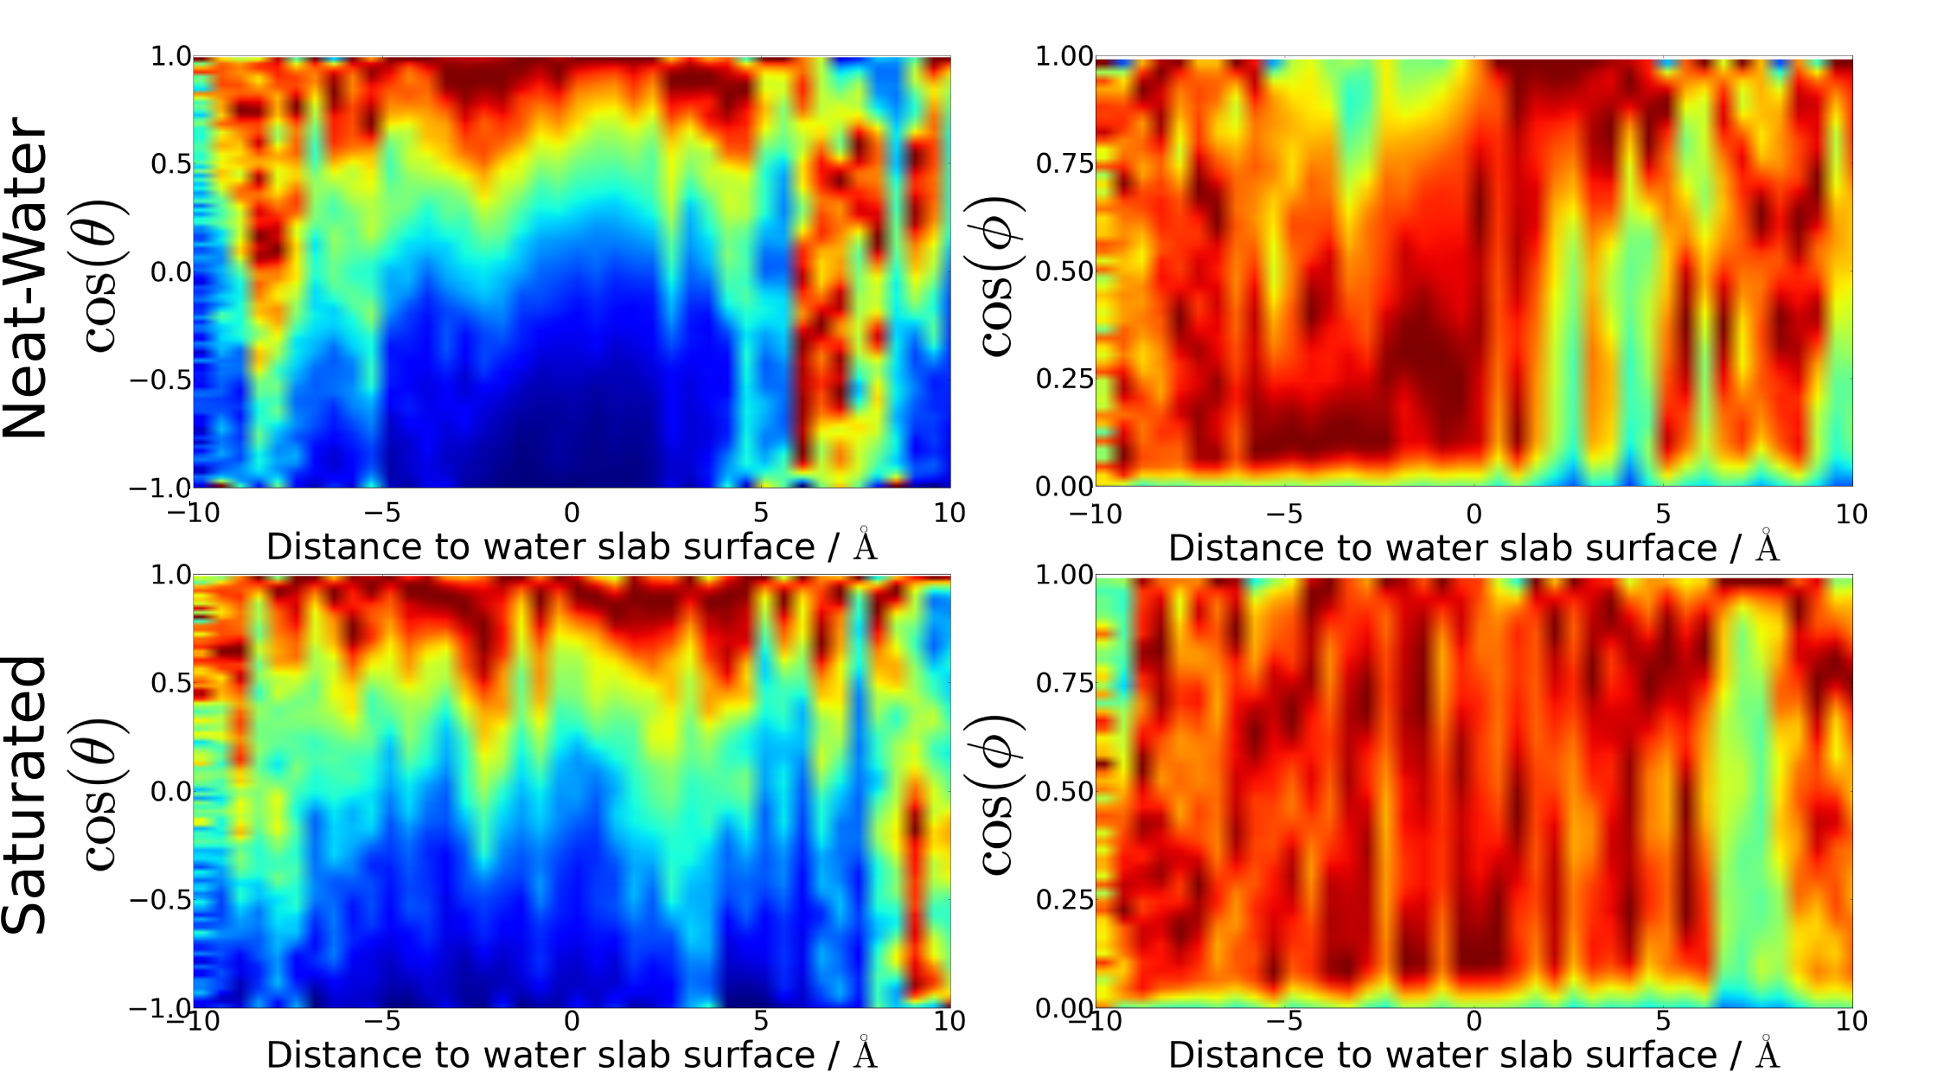
\includegraphics[scale=1.0]{images/transit-so2-angles/so2-angles-transit.png}
		\caption{\suldiox~molecular orientation distributions during SMD transit simulations into an aqueous slab. Both the neat-water (top row) and saturated (bottom row) data sets were analyzed to determine the angles $\theta$ (left column), and $\phi$ (right column) of the transiting \suldiox. The distributions show angle cosines plotted against the distance of the \suldiox~to the location of the water surface. The data sets were averaged at each distance for the respective 50 simulations.}
		\label{fig:so2-transit-angles}
	\end{center}
\end{figure}

	From its starting position 20\angs above the water surface, until the \suldiox~moves to within 10\angs of the surface of both systems, the orientation is isotropic in $\phi$. The trend for the bisector angle, $\theta$, upon approaching the surface is to become more perpendicular to the surface with the \suldiox~sulfur pointing into the water phase. At the point when the \suldiox~reaches the surface location (distance$=0$), the bisector is mostly perpendicular in both the neat-water and saturated systems. In the distribution of $\phi$, both systems show isotropy in the orientation
 
  Upon approaching the saturated surface at approx. 5\angs, the \suldiox~$\phi$ orientation distribution begins to cluster near $\cos(\phi)=1$, with the $\theta$ distribution remaining more isotropic, but with a trend of $\cos(\theta)>0$. At 5\angs the \suldiox~begins interacting with the other \suldiox~molecules that sit atop the water, and the resulting orientation distribution suggests that contact with the \suldiox~layer causes the adsorbing molecule to lie more flat to the surface. Within this same region from 0-5\angs above the surface, the $\phi$ distribution of the neat-\wat~system remains isotropic. The intensity of the distribution (darker blue) also indicates that the \suldiox~spends little time in this region, as it is quickly adsorbed further into the water bulk.

	%Just below the water surface as the distance moves into negative values, both systems show clear orientational preferences. In both systems the bisector orientation clusters such that $\cos(\theta)<0.5$, with most of the distribution intensity around $\cos(\theta)=1$. This suggests that \suldiox~in a water surface orients with the sulfur pointing into the water bulk, and the oxygens pointing towards the surface water molecules.

	%Differences occurr between the system orientation profiles once the \suldiox~has moved further than 10\angs below the surface. While both $\theta$ and $\phi$ hold the same trend from just under the surface through to the bulk of the slab in the saturated system, the orientation profile becomes much more isotropic past 10\angs under the surface of the neat-\wat~system. The orientation effect is shallower under the neat-\wat~surface. However, the orientation distribution peaks most intensely, and more tightly clustered with the \suldiox~bisector aligning with the surface normal, just underneath the neat-\wat~surface than the saturated one. The distributions thus show an orienting force extending deeper into the surface of the saturated system than the neat-\wat~system. In terms of how deeply the \suldiox~molecule is oriented, the interfacial region of the saturated system is larger and extends further into the aqueous bulk.
